\vspace{-15pt}
\section{Introduction}
Deep neural models based on Convolutional Neural Networks (CNNs)
have enabled unprecedented breakthroughs in a variety of computer vision tasks, from image
classification~\cite{krizhevsky_nips12,he_cvpr15}, object detection~\cite{girshick2014rcnn}, semantic segmentation~\cite{long2015fcn} to image captioning~\cite{vinyals_cvpr15,chen2015microsoft,fang2015captions,johnson_cvpr16}, visual question answering~\cite{antol2015vqa,gao2015you,malinowski_iccv15,ren_nips15}
and more recently, visual dialog~\cite{visdial,guesswhat,visdial_rl} and
embodied question answering~\cite{embodiedqa,gordon2017iqa}.
While these models enable superior performance, their lack of decomposability into
\emph{individually intuitive} components makes them hard to interpret~\cite{lipton_arxiv16}.
Consequently, when today's intelligent systems fail, they often fail spectacularly disgracefully
without warning or explanation, leaving a user staring at an incoherent output, wondering why the system did what it did.  %


\emph{Interpretability matters.}
In order to build trust in intelligent systems and move towards their meaningful
integration into our everyday lives,
it is clear that we must build `transparent' models that have the ability to
explain \emph{why they predict what they \rama{predict}}.
Broadly speaking, this transparency and ability to explain is useful at three different stages of Artificial Intelligence (AI) evolution.
First, when AI is significantly weaker than humans and not yet reliably deployable (\eg visual question
answering ~\cite{antol2015vqa}), the goal of transparency and explanations is to identify the failure
modes~\cite{agrawal2016analyzing,hoiem2012diagnosing}, thereby helping researchers focus their
efforts on the most fruitful research directions.
Second, when AI is on par with humans and reliably deployable (\eg, image classification~\cite{karpathy_imagenet}
trained on sufficient data), the goal
is to establish appropriate trust \rama{and confidence in} users.
Third, when AI is significantly stronger than humans (\eg chess or Go~\cite{silver2016mastering}),
the goal of explanations is \rama{in} machine teaching~\cite{JohnsCVPR2015} -- \ie, a
machine teaching a human about how to make better decisions.%




\begin{figure*}[t!]
	\centering
	\begin{subfigure}[t]{0.161\textwidth}
		\centering
		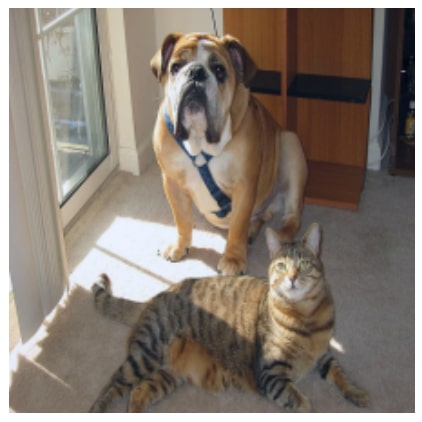
\includegraphics[width=\textwidth]{figures/teaser/original.jpg}
        \caption{\scriptsize{Original Image}}
	\end{subfigure}
	\begin{subfigure}[t]{0.161\textwidth}
		\centering
		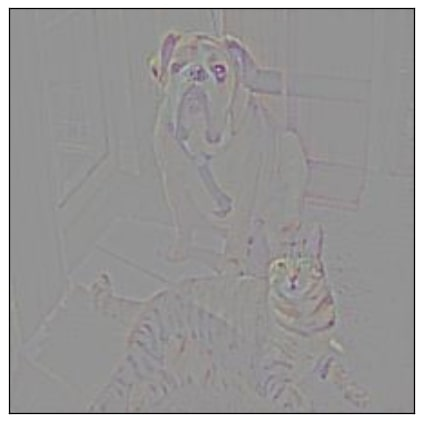
\includegraphics[width=\textwidth]{figures/teaser/gb.jpg}
        \caption{\scriptsize{Guided Backprop `Cat'}}
        \label{fig:teaser_gb_cat}
	\end{subfigure}
	\begin{subfigure}[t]{0.161\textwidth}
		\centering
		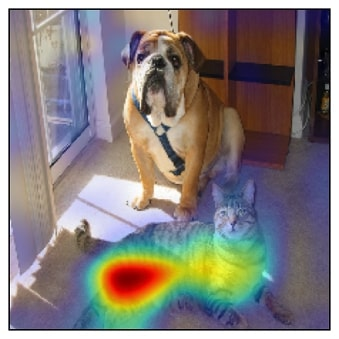
\includegraphics[width=\textwidth]{figures/teaser/newgcam_heatmap_overlaid_283_cat_dog_with_margin_small.jpg}
        \caption{\scriptsize{Grad-CAM `Cat'}}
        \label{fig:teaser_gcam_cat}
	\end{subfigure}
	\begin{subfigure}[t]{0.161\textwidth}
		\centering
		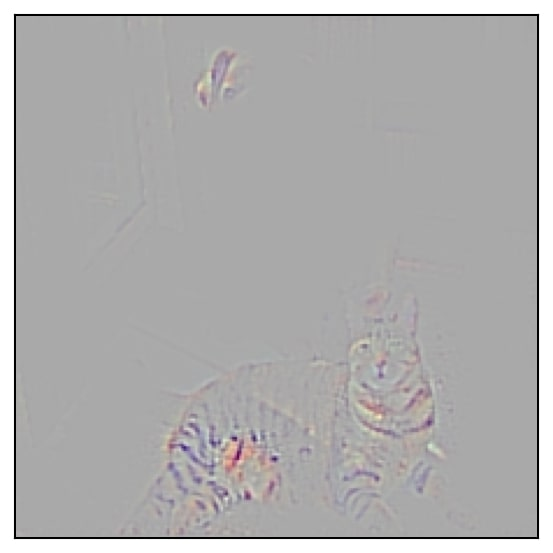
\includegraphics[width=0.995\textwidth]{figures/teaser/gbgcam_cat_margin.jpg}
        \caption{\hspace{-1.5pt}\scriptsize{Guided Grad-CAM `Cat'}}
        \label{fig:teaser_gbgcam_cat}
	\end{subfigure}
	\begin{subfigure}[t]{0.161\textwidth}
		\centering
		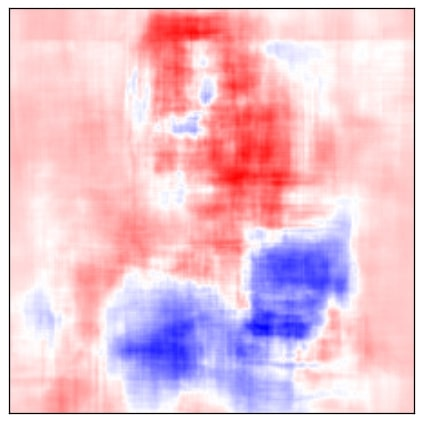
\includegraphics[width=\textwidth]{figures/teaser/occlusion.jpg}
        \caption{\scriptsize{Occlusion map `Cat'}}
        \label{fig:teaser_cat_occlusion}
	\end{subfigure}
	\begin{subfigure}[t]{0.161\textwidth}
		\centering
		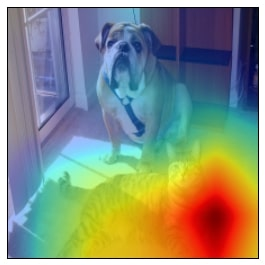
\includegraphics[width=0.995\textwidth]{figures/gcam_res18_283.jpg}
		\caption{\scriptsize{ResNet \gcam{} `Cat'}}
        \label{fig:teaser_cat_occlusion}
	\end{subfigure}\\
    \vspace*{10pt}
	\begin{subfigure}[t]{0.161\textwidth}
		\centering
        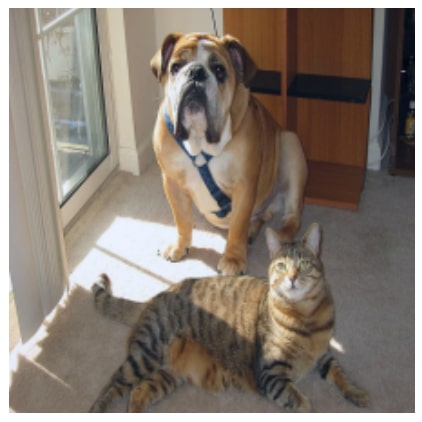
\includegraphics[width=\textwidth]{figures/teaser/original.jpg}
        \caption{\scriptsize{Original Image}\hspace{-12pt}}
	\end{subfigure}
	\begin{subfigure}[t]{0.161\textwidth}
		\centering
        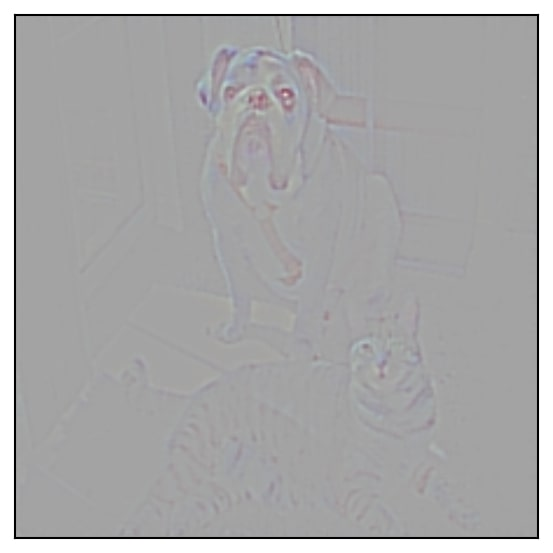
\includegraphics[width=\textwidth]{figures/teaser/dog_gb.jpg}
		\caption{\scriptsize{Guided Backprop `Dog'}\hspace{-12pt}}
        \label{fig:teaser_gb_dog}
	\end{subfigure}
	\begin{subfigure}[t]{0.161\textwidth}
		\centering
        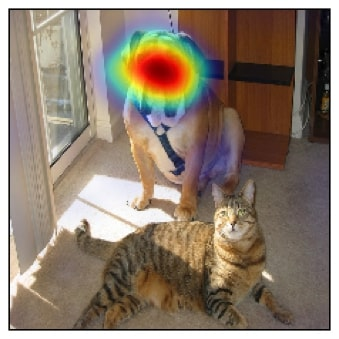
\includegraphics[width=\textwidth]{figures/teaser/newgcam_heatmap_overlaid_243_cat_dog_with_margin_small.jpg}
        \caption{\scriptsize{Grad-CAM `Dog'}\hspace{-12pt}}
        \label{fig:teaser_gcam_dog}
	\end{subfigure}
	\begin{subfigure}[t]{0.161\textwidth}
		\centering
        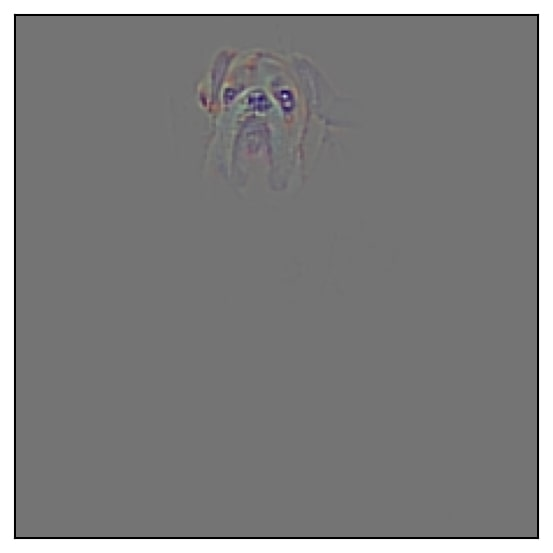
\includegraphics[width=1.01\textwidth]{figures/teaser/gbgcam_dog_margin.jpg}
        \caption{\hspace{-1.9pt}\scriptsize{Guided Grad-CAM `Dog'}\hspace{-12pt}}
        \label{fig:teaser_gbgcam_dog}
	\end{subfigure}
	\begin{subfigure}[t]{0.161\textwidth}
		\centering
        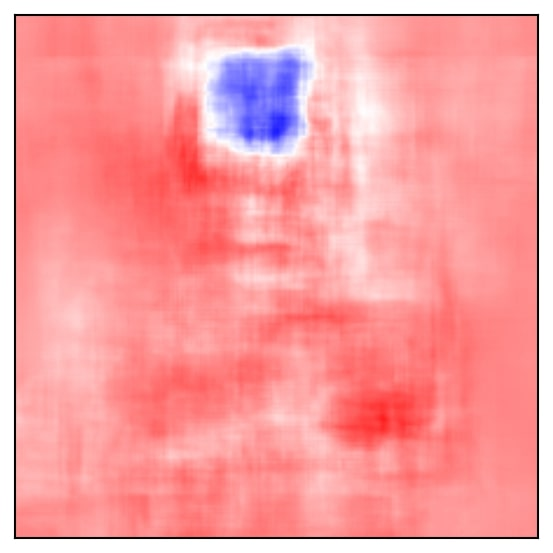
\includegraphics[width=\textwidth]{figures/teaser/dog_occlusion.jpg}
        \caption{\scriptsize{Occlusion map `Dog'}\hspace{-12pt}}
        \label{fig:teaser_dog_occlusion}
	\end{subfigure}
	\begin{subfigure}[t]{0.161\textwidth}
		\centering
		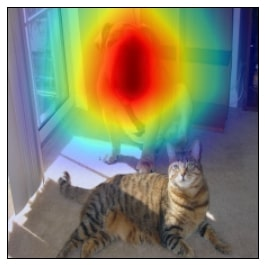
\includegraphics[width=0.995\textwidth]{figures/gcam_res18_243.jpg}
		\caption{\hspace{-1.9pt}\scriptsize{ResNet \gcam{} `Dog'}}
        \label{fig:teaser_gcam_resnet}
	\end{subfigure}
    \vspace{14pt}
	\caption{
		(a) Original image with a cat and a dog. (b-f) Support for the cat category according to various visualizations \rp{for VGG-16 and ResNet}.
		(b) Guided Backpropagation~\cite{springenberg_arxiv14}: highlights all contributing features. (c, f) \gcam{} (Ours): localizes class-discriminative regions, (d) Combining (b) and (c) gives Guided Grad-CAM, which gives high-resolution class-discriminative visualizations. %
		Interestingly, the localizations achieved by our \gcam{} technique, (c) are very similar to results from occlusion sensitivity (e), while being orders of magnitude cheaper to compute. (f, l) are \gcam{} visualizations for ResNet-18 layer.
		Note that in (c, f, i, l), red regions corresponds to high score for class, while in (e, k), blue corresponds to evidence for the class.
		Figure best viewed in color.
	  }
    \label{fig:teaser}
\end{figure*}

There typically exists a trade-off between accuracy and simplicity or interpretability.
Classical rule-based or expert systems~\cite{jackson_expertsys} are highly interpretable but not very accurate (or robust).
Decomposable pipelines where each stage is hand-designed are thought to be more interpretable as each individual component assumes a natural intuitive explanation.
By using deep models, we sacrifice interpretable modules for uninterpretable ones that achieve greater performance through greater abstraction (more layers) and tighter integration (end-to-end training). Recently introduced deep residual networks (ResNets)~\cite{he_cvpr15} are over 200-layers deep and have shown state-of-the-art performance in several challenging tasks. \rama{
Such complexity makes these models hard to interpret.}
As such, deep models are beginning to explore the spectrum between interpretability and accuracy.

\rpr{Zhou~\etal~\cite{zhou_cvpr16} recently proposed a technique called Class Activation Mapping (CAM) for identifying discriminative regions used by a restricted class of image classification CNNs which do not contain any fully-connected layers.
  In essence, this work trades off model complexity and performance for more transparency into the working of the model.
In contrast, we make existing state-of-the-art deep models interpretable without altering their architecture, thus \rama{avoiding the interpretability \vs accuracy trade-off}.
Our approach is a generalization of CAM~\cite{zhou_cvpr16} and is applicable to a significantly broader range of CNN model families: (1) CNNs with fully-connected layers (\eg VGG), (2) CNNs used for structured outputs (\eg captioning), (3) CNNs used in tasks with multi-modal inputs (\eg VQA) or reinforcement learning, without requiring architectural changes or re-training. %
}






\noindent \textbf{What makes a good visual explanation?}
Consider image classification~\cite{imagenet_cvpr09} -- a `good’ visual explanation from the model for justifying any target category should be (a) class-discriminative (\ie localize the category in the image) and (b) high-resolution (\ie capture fine-grained detail).

Fig.~\hyperlink{page.2}{1} shows outputs from a number of visualizations for the `tiger cat' class (top) and `boxer' (dog) class (bottom).
\mac{Pixel-space gradient visualizations such as \gb{}~\cite{springenberg_arxiv14}  and \dec{}~\cite{zeiler_eccv14}
are high-resolution and highlight fine-grained details in the image, but are not class-discriminative
(\figref{fig:teaser_gb_cat} and \figref{fig:teaser_gb_dog} are very similar).}



\mac{In contrast, localization approaches like CAM or our proposed method Gradient-weighted Class Activation Mapping (\gcam{}),
are highly class-discriminative
(the `cat' explanation exclusively highlights the `cat' regions but not `dog' regions in \figref{fig:teaser_gcam_cat}, and \viceversa{} in \figref{fig:teaser_gcam_dog}).
}

In order to combine the best of both worlds, we show that it is possible to fuse existing pixel-space gradient visualizations with \gcam{} to create \cgb{} visualizations that are both high-resolution and class-discriminative. As a result, important regions of the image which correspond to any decision of interest are visualized in high-resolution detail even if the image contains \rp{evidence for multiple possible} \rama{concepts}, as shown in Figures \hyperlink{page.2}{1d} and \hyperlink{page.2}{1j}.
When visualized for `tiger cat', \cgb{} not only highlights the cat regions, but also highlights the stripes on the cat, which is important for predicting that particular variety of cat.
















\noindent To summarize, our contributions are as follows:

\noindent \textbf{(1)}
\mac{We introduce \gcam{}, a class-discriminative localization technique that generates
visual explanations for \emph{any} CNN-based network without requiring architectural changes or re-training.
We evaluate \gcam{} for localization (\secref{sec:localization}), and faithfulness to model (\secref{sec:occ}), where it outperforms baselines.}

\noindent \textbf{(2)}
\mac{We apply \gcam{} to existing top-performing classification, captioning (\secref{sec:nic}), and VQA (\secref{sec:vqa}) models.}
For image classification, our visualizations lend insight into failures of current CNNs (\secref{sec:diagnose}), showing that seemingly unreasonable predictions have reasonable explanations.
For captioning and VQA, our visualizations expose
that common \mac{CNN + LSTM models are often surprisingly good at}
localizing discriminative image regions despite not being trained on
grounded image-text pairs.

\noindent \textbf{(3)}
We show a proof-of-concept of how interpretable \gcam{} visualizations
help in diagnosing failure modes by uncovering biases in datasets.
This is important not just for generalization, but also for fair and
bias-free outcomes as more and more decisions are made by algorithms in society.

\noindent \textbf{(4)}
We present Grad-CAM visualizations for ResNets~\cite{he_cvpr15} applied to
image classification and VQA (\secref{sec:vqa}).

\ijcv{\noindent \textbf{(5)}
We use neuron importance from \gcam{} and neuron names from~\cite{netdissect} and obtain textual explanations for model decisions (\secref{sec:text_exp}).}

\noindent \textbf{(6)}
We conduct human studies (\secref{sec:human_evaluation}) \mac{that show \cgb{} explanations are class-discriminative and not only help humans establish trust,
but also help untrained users successfully discern a `stronger' network from a `weaker' one,
\emph{even when both make identical predictions.}}




\rpi{\noindent \textbf{Paper Organization: }
The rest of the paper is organized as follows. 
In section 3 we propose our approach \gcam{} and \cgb{}. 
In sections 4 and 5 we evaluate the localization ability, class-discriminativeness, trustworthyness and faithfulness of \gcam{}. 
In section 6 we show certain use cases of \gcam{} such as diagnosing image classification CNNs and identifying biases in datasets. 
In section 7 we provide a way to obtain textual explanations with \gcam{}. 
In section 8 we show how \gcam{} can be applied to vision and language models -- image captioning and Visual Question Answering (VQA).}


\begin{figure*}
    \begin{center}
  \centering
  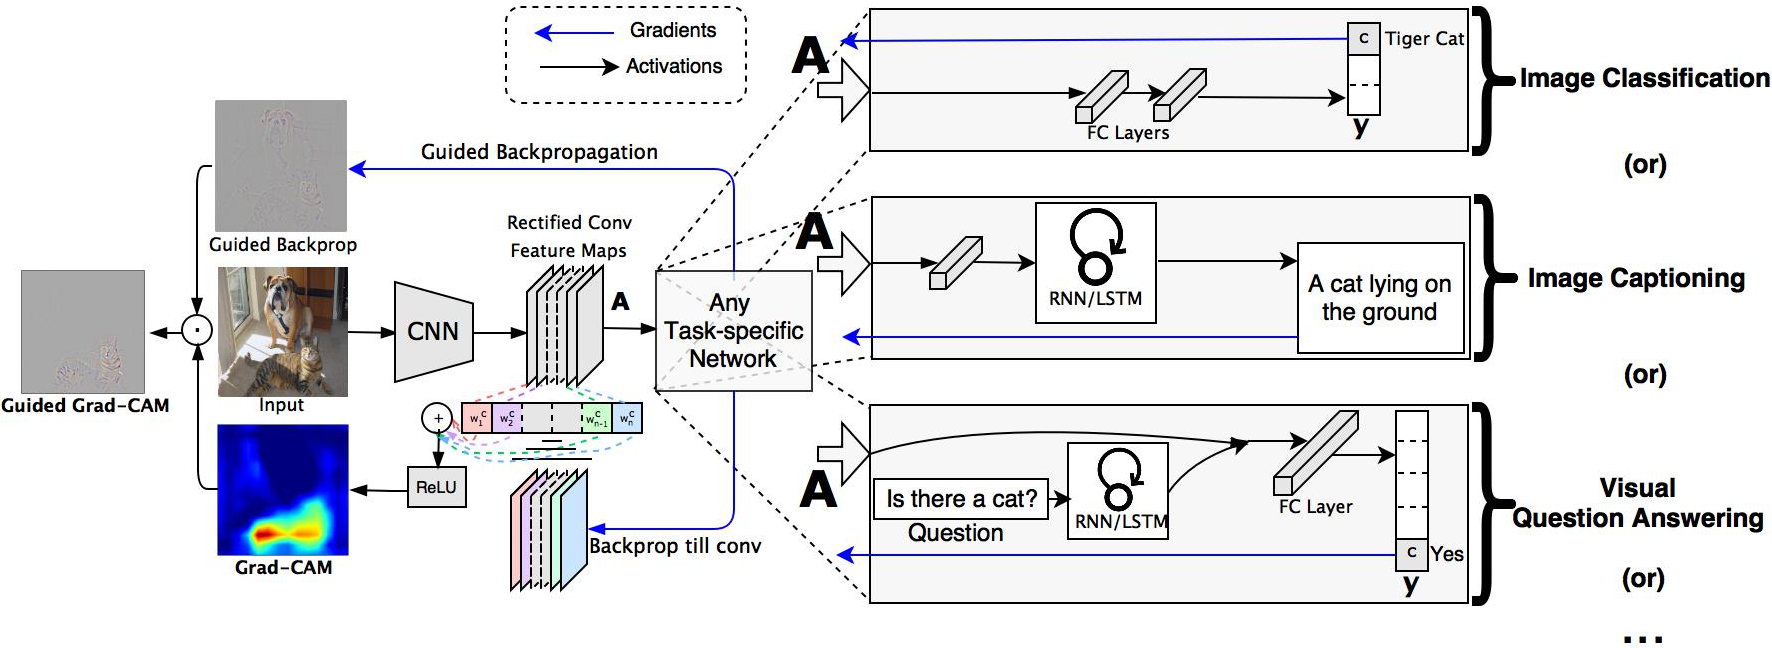
\includegraphics[width=\textwidth]{figures/Grad-CAM_approach.png}
	\caption{\scriptsize  \gcam{} overview: Given an image \mac{ and a class of interest (\eg, `tiger cat' or any other type of differentiable output) as input, we forward propagate the image through the CNN part of the model and then through task-specific computations to obtain a raw score for the category.}
        The gradients are set to zero for all classes except the desired class (tiger cat), which is set to 1.
		This signal is then backpropagated to the rectified convolutional \mac{feature maps of interest, which we combine to compute} the coarse \gcam{} localization (blue heatmap) \rp{which represents where the model has to look to make the particular decision}.
	Finally, we pointwise multiply the heatmap with guided backpropagation to get \cgb{} visualizations which are both high-resolution and concept-specific.
}
	\label{fig:approach}
\end{center}
\end{figure*}

